With the piecewise-linear representations of the power spectrum and the kernel functions established in Section~\ref{sec:4}, we now cast the Limber integral (Equation~\ref{eq:2.1}) into a tensorised form that cleanly separates cosmology-dependent integrals from survey-dependent redshift distributions. This factorisation is the central result of the paper and the foundation of the \texttt{LimberCloud} framework.

The first step is to decompose the continuous line-of-sight integral into a sum of integrals over the \(N_\mathrm{Z}\) comoving-distance intervals \([\chi_n, \chi_{n+1}]\) defined by the redshift grid. For a generic tracer pair \((u, v)\) in tomographic bins \((a, b)\), Equation~\ref{eq:2.1} becomes
\begin{equation} \label{eq:5.1}
    C_{uv}^{ab}(\ell) = A_{uv}(\ell) \sum_{n=0}^{N_\mathrm{Z}-1} \int_{\chi_n}^{\chi_{n+1}} \mathrm{d}\chi\; \frac{W_u^{a,n}(\chi)\,W_v^{b,n}(\chi)}{\chi^2}\, P_{uv}\!\left[\frac{\ell + 1/2}{\chi},\, z(\chi)\right],
\end{equation}
where the flat-sky simplification \(f_K(\chi) = \chi\) has been applied and the superscript \(n\) on each kernel restricts it to the \(n\)-th comoving-distance interval, following the convention introduced in Section~\ref{sec:4.2}. The multipole-dependent prefactor \(A_{uv}(\ell)\) accounts for the spin of the projected fields and is specified for each tracer pair in Table~\ref{tab:1}.

The key insight of the tensorised reformulation is that, within each interval, both kernels admit the decomposition derived in Section~\ref{sec:4}. For the number-density kernel and the lensing convergence kernel respectively,
\begin{equation} \label{eq:5.2}
    W_\phi^{a,n}(\chi) = \sum_{i=0}^{N_\mathrm{Z}} r_\phi^{i,n}(\chi)\,\phi^{a}_{i}, \qquad
    W_\kappa^{a,n}(\chi) = \sum_{i=0}^{N_\mathrm{Z}} r_\kappa^{i,n}(\chi)\,\phi^{a}_{i},
\end{equation}
where the coefficients \(r_\phi^{i,n}\) and \(r_\kappa^{i,n}\) depend only on cosmology and the redshift grid, while the discretised redshift distributions \(\phi^{a}_{i}\) encode all survey-specific information. Denoting the kernel type associated with tracer \(u\) generically by \(r_u^{i,n}\)---standing for either \(r_\phi^{i,n}\) or \(r_\kappa^{i,n}\) as specified in Table~\ref{tab:1}---substituting Equation~\ref{eq:5.2} together with the linearised power spectrum (Equation~\ref{eq:4.1}) into Equation~\ref{eq:5.1} yields
\begin{equation} \label{eq:5.3}
    C_{uv}^{ab}(\ell) = A_{uv}(\ell) \sum_{n=0}^{N_\mathrm{Z}-1} \sum_{i=0}^{N_\mathrm{Z}} \sum_{j=0}^{N_\mathrm{Z}} \left[\int_{\chi_n}^{\chi_{n+1}} \mathrm{d}\chi\; \frac{r_u^{i,n}(\chi)\,r_v^{j,n}(\chi)}{\chi^2}\, P_{uv}\!\left[\frac{\ell+1/2}{\chi},\, z(\chi)\right]\right] \phi^{a}_{i}\,\phi^{b}_{j}.
\end{equation}
Since the redshift distribution values \(\phi^{a}_{i}\) and \(\phi^{b}_{j}\) are independent of both \(\chi\) and the interval index \(n\), they factor out of the integral and the sum over intervals. This motivates the definition of the \emph{interval tensor},
\begin{equation} \label{eq:5.4}
    B_{uv}^{ij,n}(\ell) \equiv A_{uv}(\ell) \int_{\chi_n}^{\chi_{n+1}} \mathrm{d}\chi\; \frac{r_u^{i,n}(\chi)\,r_v^{j,n}(\chi)}{\chi^2}\, P_{uv}\!\left[\frac{\ell+1/2}{\chi},\, z(\chi)\right],
\end{equation}
which encapsulates all cosmology- and geometry-dependent information within a single redshift interval. Summing over intervals defines the \emph{basis tensor},
\begin{equation} \label{eq:5.5}
    B_{uv}^{ij}(\ell) \equiv \sum_{n=0}^{N_\mathrm{Z}-1} B_{uv}^{ij,n}(\ell),
\end{equation}
so that the angular power spectrum reduces to a compact double contraction,
\begin{equation} \label{eq:5.6}
    \boxed{C_{uv}^{ab}(\ell) = \sum_{i=0}^{N_\mathrm{Z}} \sum_{j=0}^{N_\mathrm{Z}} B_{uv}^{ij}(\ell)\,\phi^{a}_{i}\,\phi^{b}_{j}.}
\end{equation}
Equation~\ref{eq:5.6} is the principal result of this work. It expresses every angular power spectrum in the \(3\times2\,\mathrm{pt}\) data vector as a bilinear form in the discretised redshift distributions, contracted against a basis tensor \(B_{uv}^{ij}(\ell)\) that depends only on cosmological parameters and the redshift grid. Crucially, the basis tensor is independent of the tomographic bin assignments: once \(B_{uv}^{ij}(\ell)\) has been computed for a given cosmology and multipole, the angular power spectra for any pair of tomographic bins are obtained by a single matrix--vector contraction with the appropriate redshift distributions. This separation provides a substantial computational advantage whenever the redshift distributions are varied---for instance during self-calibration of photometric redshift uncertainties---because only the outer contraction in Equation~\ref{eq:5.6} needs to be re-evaluated, while the expensive integral (Equation~\ref{eq:5.4}) remains unchanged.

The interval tensor \(B_{uv}^{ij,n}(\ell)\) defined in Equation~\ref{eq:5.4} involves a product of two piecewise-linear kernel coefficients and the linearised power spectrum, all of which are at most linear in \(\chi\) within each interval. The resulting integrand is a rational function of \(\chi\)---with additional logarithmic terms whenever the lensing convergence coefficient \(r_\kappa^{i,n}\) participates---that admits a closed-form evaluation in every case. All closed-form expressions were derived using computer algebra (\texttt{Mathematica}) and independently verified against direct numerical quadrature.

The structure of \(B_{uv}^{ij,n}(\ell)\) is determined by which kernel types appear on each leg of the tracer pair (Table~\ref{tab:1}), giving rise to three structural cases, each characterised by a distinct set of closed-form integral formulas. When both kernels are of number-density type (\(r_\phi \times r_\phi\)), the sparsity of \(r_\phi^{i,n}\)---non-zero only for \(i \in \{n, n{+}1\}\) (Equation~\ref{eq:4.5})---limits the non-vanishing entries to three structurally distinct index configurations per interval, \((i,j) \in \{(n,n),\, (n,n{+}1),\, (n{+}1,n{+}1)\}\), after accounting for the symmetry \(B_{uv}^{ij,n} = B_{uv}^{ji,n}\). When one kernel is of number-density type and the other of lensing convergence type (\(r_\phi \times r_\kappa\)), the first index retains the two-point support while the second spans the four structural cases of \(r_\kappa^{j,n}\) (Equations~\ref{eq:4.9a}--\ref{eq:4.9d}), yielding \(2 \times 4 = 8\) distinct analytic formulas per interval. Because the general structural case (Equation~\ref{eq:4.9c}) covers all intermediate grid points \(n{+}1 < j < N_\mathrm{Z}\) with a single functional form, these eight formulas suffice to evaluate the \(\mathcal{O}(N)\) non-zero entries of the mixed tensor at each interval. When both kernels are of lensing convergence type (\(r_\kappa \times r_\kappa\)), both indices span the four structural cases, producing ten unique formulas after symmetry reduction. In total, 21 structurally distinct analytic integral formulas per redshift interval are required to populate the full basis tensor for the complete \(3\times2\,\mathrm{pt}\) data vector; each is implemented as a separate function in \texttt{LimberCloud}.

The bin-independence of the basis tensor relies on the assumption that the three-dimensional power spectrum, \(P_{uv}(k,z)\), and hence any bias functions it absorbs (Table~\ref{tab:1}), does not depend on the tomographic bin assignment. Three regimes can be distinguished. First, if the bias function is determined entirely by \((k,z)\) and is the same for all bins---as is the case for intrinsic alignments under the non-linear alignment (NLA) model, where \(b_\mathrm{I}(z) \propto -A_\mathrm{IA}\,C_1\,\rho_\mathrm{cr}\,\Omega_\mathrm{m}/D(z)\)---the factorisation holds exactly and the basis tensor is computed once per tracer pair. Second, if the bias varies across tomographic bins but is constant within each bin---the standard parameterisation for galaxy bias, which assigns a free amplitude \(b_\mathrm{g}^{a}\) to each lens bin---the per-bin constants factor out of the integral and can be absorbed into modified distributions \(\tilde{\phi}^{a}_{i} = b_\mathrm{g}^{a}\,\phi^{a}_{i}\), so that the basis tensor again needs to be evaluated only once (using \(P_{\delta\delta}\) in place of \(b_\mathrm{g}^{2}\,P_{\delta\delta}\)); the magnification response \(b_\mu^{a}\), being a constant per lens bin, is treated identically. Third, if the bias depends on both \((k,z)\) and varies across bins---for example a scale-dependent galaxy bias \(b_\mathrm{g}^{a}(k,z)\) that differs between tomographic selections---the bias cannot be factored out of Equation~\ref{eq:5.4} and a separate basis tensor must be computed for each bin pair, substantially increasing the computational cost. The first two regimes encompass the bias models most commonly adopted in current Stage-IV \(3\times2\,\mathrm{pt}\) analyses, including those assumed throughout this work (Section~\ref{sec:3}). Analyses that incorporate beyond-linear, scale-dependent galaxy bias models varying across tomographic selections would enter the third regime; such models are not yet standard but may become relevant as survey precision increases. In either case, the tensorised factorisation remains applicable---only the computational cost of evaluating the basis tensor changes, as discussed further in Section~\ref{sec:6.2}.

We now validate the tensorised formulation for each of the three combined observables defined in Equations~\ref{eq:2.5}--\ref{eq:2.7}: the shape--shape correlation \(C_{\epsilon\epsilon}^{ab}(\ell)\), the position--shape correlation \(C_{\theta\epsilon}^{ab}(\ell)\), and the position--position correlation \(C_{\theta\theta}^{ab}(\ell)\). In each case, the full observable is obtained by computing the basis tensor \(B_{uv}^{ij}(\ell)\) for every constituent tracer pair listed in Table~\ref{tab:1} and summing the resulting angular power spectra according to Equations~\ref{eq:2.5}--\ref{eq:2.7}. The combined spectra are then compared with the direct numerical evaluation by \texttt{CCL}.

\subsection{Shape--shape correlation} \label{sec:5.1}

The shape--shape angular power spectrum \(C_{\epsilon\epsilon}^{ab}(\ell)\) receives contributions from gravitational lensing, intrinsic alignments, and their cross-terms (Equation~\ref{eq:2.5}). For the dominant pure-lensing contribution \(C_{\gamma\gamma}^{ab}(\ell)\), both kernels are of lensing convergence type and the spin-2 prefactor is \(A_{\gamma\gamma}(\ell) = (\ell+2)!/[(\ell-2)!\,(\ell+1/2)^4]\). The interval tensor is
\begin{equation} \label{eq:5.7}
    B_{\gamma\gamma}^{ij,n}(\ell) = A_{\gamma\gamma}(\ell) \int_{\chi_n}^{\chi_{n+1}} \mathrm{d}\chi\; \frac{r_\kappa^{i,n}(\chi)\,r_\kappa^{j,n}(\chi)}{\chi^2}\, P_{\delta\delta}\!\left[\frac{\ell+1/2}{\chi},\, z(\chi)\right],
\end{equation}
which is dense in both indices, requiring ten unique coefficient elements per interval. The intrinsic-alignment cross-terms \(C_{\gamma\mathrm{I}}^{ab}(\ell)\) and \(C_{\mathrm{I}\gamma}^{ab}(\ell)\) each involve one lensing kernel and one number-density kernel, with \(P_{\mathrm{I}\delta}(k,z) = b_\mathrm{I}(k,z)\,P_{\delta\delta}(k,z)\); by construction, \(C_{\mathrm{I}\gamma}^{ab}(\ell) = C_{\gamma\mathrm{I}}^{ba}(\ell)\), so only one of these two contributions needs to be computed independently. The pure intrinsic--intrinsic term \(C_\mathrm{II}^{ab}(\ell)\) uses \(r_\phi^{i,n}\) on both legs with \(P_\mathrm{II}(k,z) = b_\mathrm{I}^2(k,z)\,P_{\delta\delta}(k,z)\), recovering the maximally sparse kernel structure with three elements per interval.

Figure~\ref{fig:5} presents the absolute fractional error \(|\delta_{\epsilon\epsilon}^{ab}(\ell)|\) of the tensorised shape--shape power spectra relative to \texttt{CCL} for all 25 source-bin combinations of the LSST Y1 survey scenario. In each panel, the dotted horizontal line marks the one per cent level (\(10^{-2}\)), and the solid curve shows the diagonal of the Gaussian covariance normalised to the fiducial spectrum, representing the expected per-bin statistical uncertainty for the survey configuration adopted in Section~\ref{sec:3}. Across all bin pairs, the \texttt{LimberCloud} error remains below the one per cent reference line over the full multipole range \(20 \le \ell \le 2000\), with typical residuals at the \(10^{-3}\) level; under the adopted survey configuration this corresponds to one to two orders of magnitude below the per-bin Gaussian covariance.

\begin{figure*}[!htbp]
    \centering
    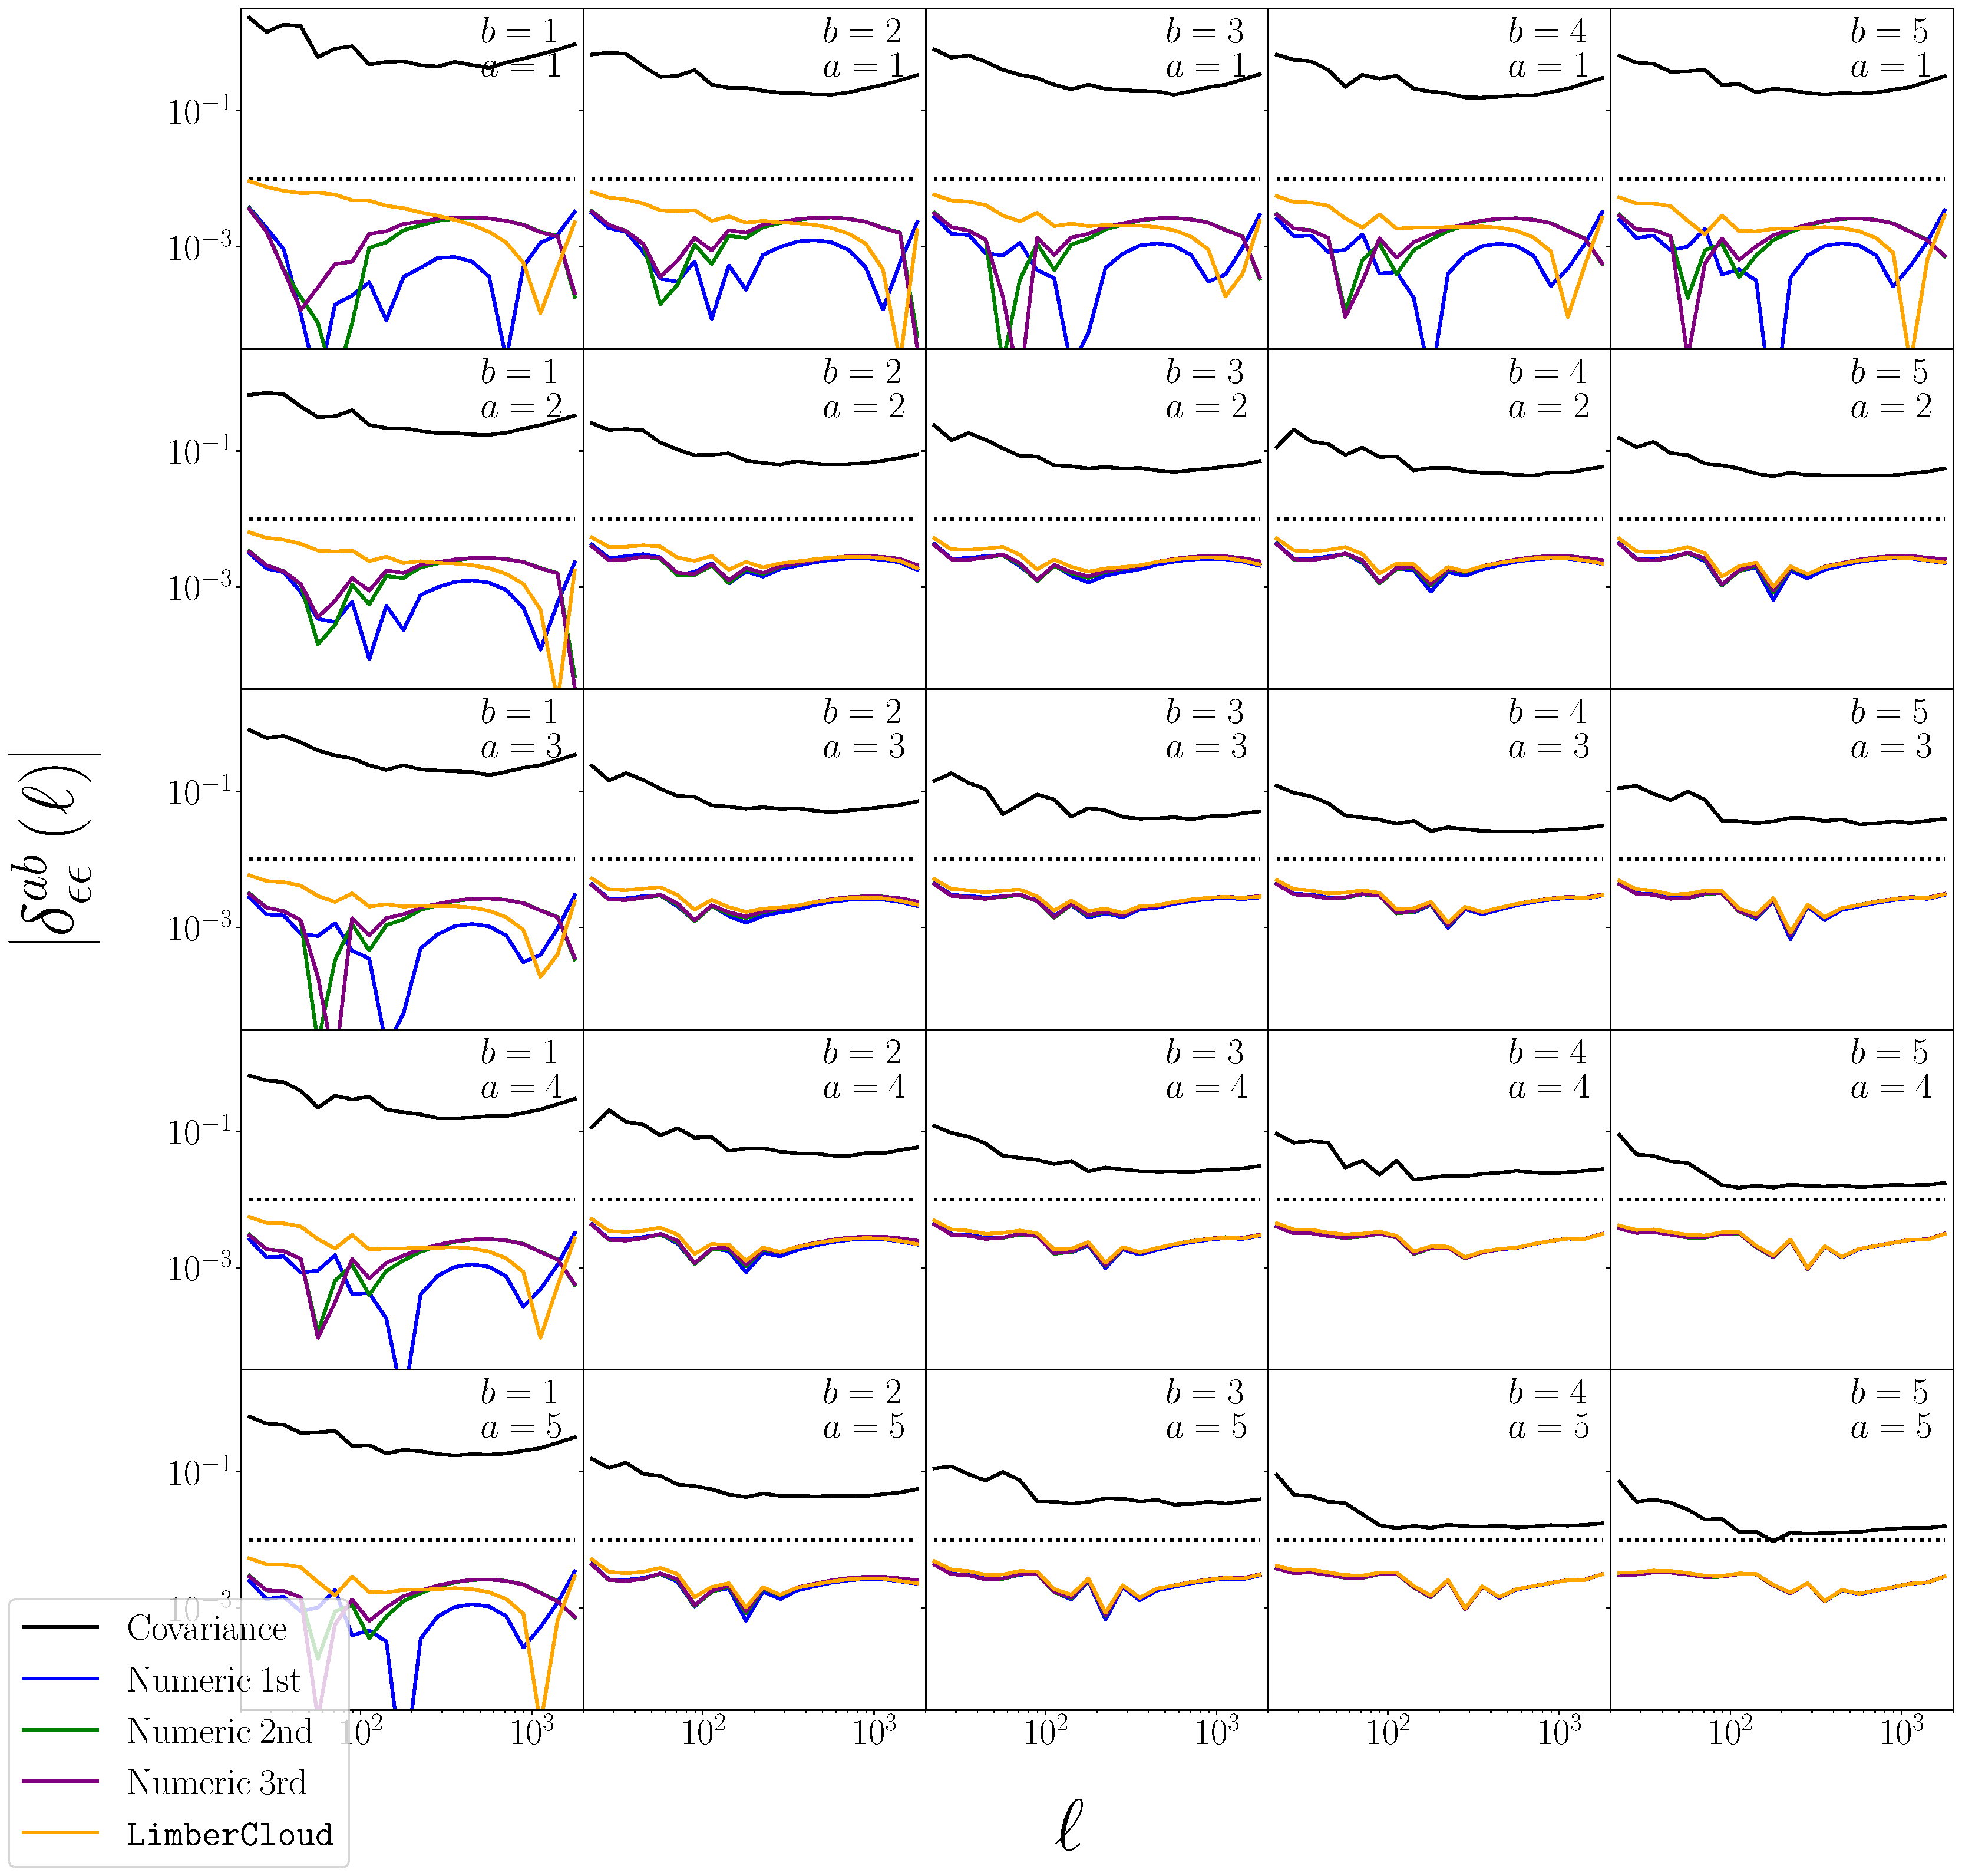
\includegraphics[width=0.95\textwidth]{figures/ERROR_EE_Y1.pdf}
    \caption{Absolute fractional error \(|\delta_{\epsilon\epsilon}^{ab}(\ell)|\) in the shape--shape (cosmic shear) angular power spectra \(C_{\epsilon\epsilon}^{ab}(\ell)\) relative to \texttt{CCL}, shown for all 25 source-bin combinations \((a, b)\) of the LSST Y1 survey scenario. Each panel corresponds to a distinct bin pair. The solid curve shows the diagonal of the Gaussian covariance normalised to the fiducial spectrum, representing the expected per-bin statistical uncertainty; the dotted horizontal line marks the one per cent level (\(10^{-2}\)). Four interpolation schemes are compared as identified in the legend: first-order numerical interpolation, second-order, third-order, and the \texttt{LimberCloud} piecewise-linear scheme. All schemes remain below the one per cent threshold for all bin combinations, with the largest residuals among auto-spectra occurring at the lowest redshifts where intrinsic-alignment contributions are relatively more important.}
    \label{fig:5}
\end{figure*}

For the auto-spectra (diagonal panels) and nearby cross-bins at intermediate to high redshifts, the fractional error lies at around the \(10^{-3}\) level. The largest residuals among the auto-spectra occur for the lowest-redshift bin pair (\(a = 1\), \(b = 1\)), where the lensing signal is intrinsically weaker and the intrinsic-alignment contributions---\(C_{\gamma\mathrm{I}}\), \(C_{\mathrm{I}\gamma}\), and \(C_\mathrm{II}\)---carry greater relative weight; partial cancellations between these terms and the dominant gravitational signal reduce the total amplitude and amplify the fractional effect of small absolute errors. A similar trend is visible for widely separated source bins (e.g.\ \(a = 1\), \(b = 5\)), where the error curves become more structured for the same reason. Notably, all four interpolation schemes track each other closely in every panel, confirming that the residual error is set primarily by the piecewise-linear power-spectrum interpolation (Equation~\ref{eq:4.1}) rather than by the kernel treatment; this observation holds across all three observables and will not be repeated below. The fractional error is generally flat or mildly increasing with \(\ell\), consistent with the expectation that the piecewise-linear approximation becomes less faithful at high multipoles where the Limber wavenumber probes more deeply non-linear scales.

\subsection{Position--shape correlation} \label{sec:5.2}

The position--shape angular power spectrum \(C_{\theta\epsilon}^{ab}(\ell)\) correlates the positions of foreground lens galaxies in bin \(a\) with the shapes of background source galaxies in bin \(b\) (Equation~\ref{eq:2.6}). For the dominant gravitational lensing contribution \(C_\mathrm{g\gamma}^{ab}(\ell)\), the number-density kernel appears on the lens leg and the lensing convergence kernel on the source leg, together with the spin-dependent prefactor \(A_\mathrm{g\gamma}(\ell) = \sqrt{(\ell+2)!/(\ell-2)!}\,/\,(\ell+1/2)^2\). The interval tensor reads
\begin{equation} \label{eq:5.8}
    B_\mathrm{g\gamma}^{ij,n}(\ell) = A_\mathrm{g\gamma}(\ell) \int_{\chi_n}^{\chi_{n+1}} \mathrm{d}\chi\; \frac{r_\phi^{i,n}(\chi)\,r_\kappa^{j,n}(\chi)}{\chi^2}\, P_\mathrm{g\delta}\!\left[\frac{\ell+1/2}{\chi},\, z(\chi)\right],
\end{equation}
where \(P_\mathrm{g\delta}(k,z) = b_\mathrm{g}(k,z)\,P_{\delta\delta}(k,z)\). Since \(r_\phi^{i,n}\) is non-zero only for \(i \in \{n, n{+}1\}\) while \(r_\kappa^{j,n}\) is non-zero for all \(j \ge n\) (Section~\ref{sec:4.3}), the tensor is sparse in the first index but dense in the second, yielding eight distinct coefficient elements per interval. The intrinsic-alignment contribution \(C_\mathrm{gI}^{ab}(\ell)\) replaces the lensing kernel with the number-density kernel on the source leg, recovering the maximally sparse three-element structure. The magnification--shear \(C_{\mu\gamma}^{ab}(\ell)\) and magnification--intrinsic \(C_{\mu\mathrm{I}}^{ab}(\ell)\) contributions follow analogously from the kernel and prefactor assignments in Table~\ref{tab:1}.

Figure~\ref{fig:6} presents the corresponding validation for the position--shape power spectra. For the majority of lens--source bin combinations, the \texttt{LimberCloud} error sits at the few \(\times\,10^{-3}\) level, well below the one per cent reference line; under the adopted survey configuration this corresponds to one to two orders of magnitude below the per-bin Gaussian covariance. A notable exception is the subset of bin pairs in which the lens and source redshift distributions overlap strongly (e.g.\ \(a = 1\), \(b = 1\) and \(a = 2\), \(b = 1\)), where the fractional error can reach \(\sim 10^{-1}\) at low multipoles. This behaviour arises because the gravitational lensing signal \(C_\mathrm{g\gamma}^{ab}\)---which requires source galaxies behind the lenses---is strongly suppressed when the two populations share the same redshift range, leaving the observable dominated by the intrinsic-alignment and magnification contributions whose partial cancellations amplify fractional residuals. In practice, these overlapping bin pairs are not conventionally included in \(3\times2\,\mathrm{pt}\) analyses, which impose a lens--source separation cut on the source leg and (in conjunction with the linear-bias scale cut discussed in Section~\ref{sec:5.3}) restrict the lens leg to multipoles where the linear-bias model is valid; their statistical uncertainties (solid curves) are correspondingly large. For all standard bin combinations, the \texttt{LimberCloud} error is comfortably below both the one per cent line and the survey variance, with a mild uptick at high \(\ell\) visible in certain cross-bins where magnification contributions become relatively more significant.

\begin{figure*}[!htbp]
    \centering
    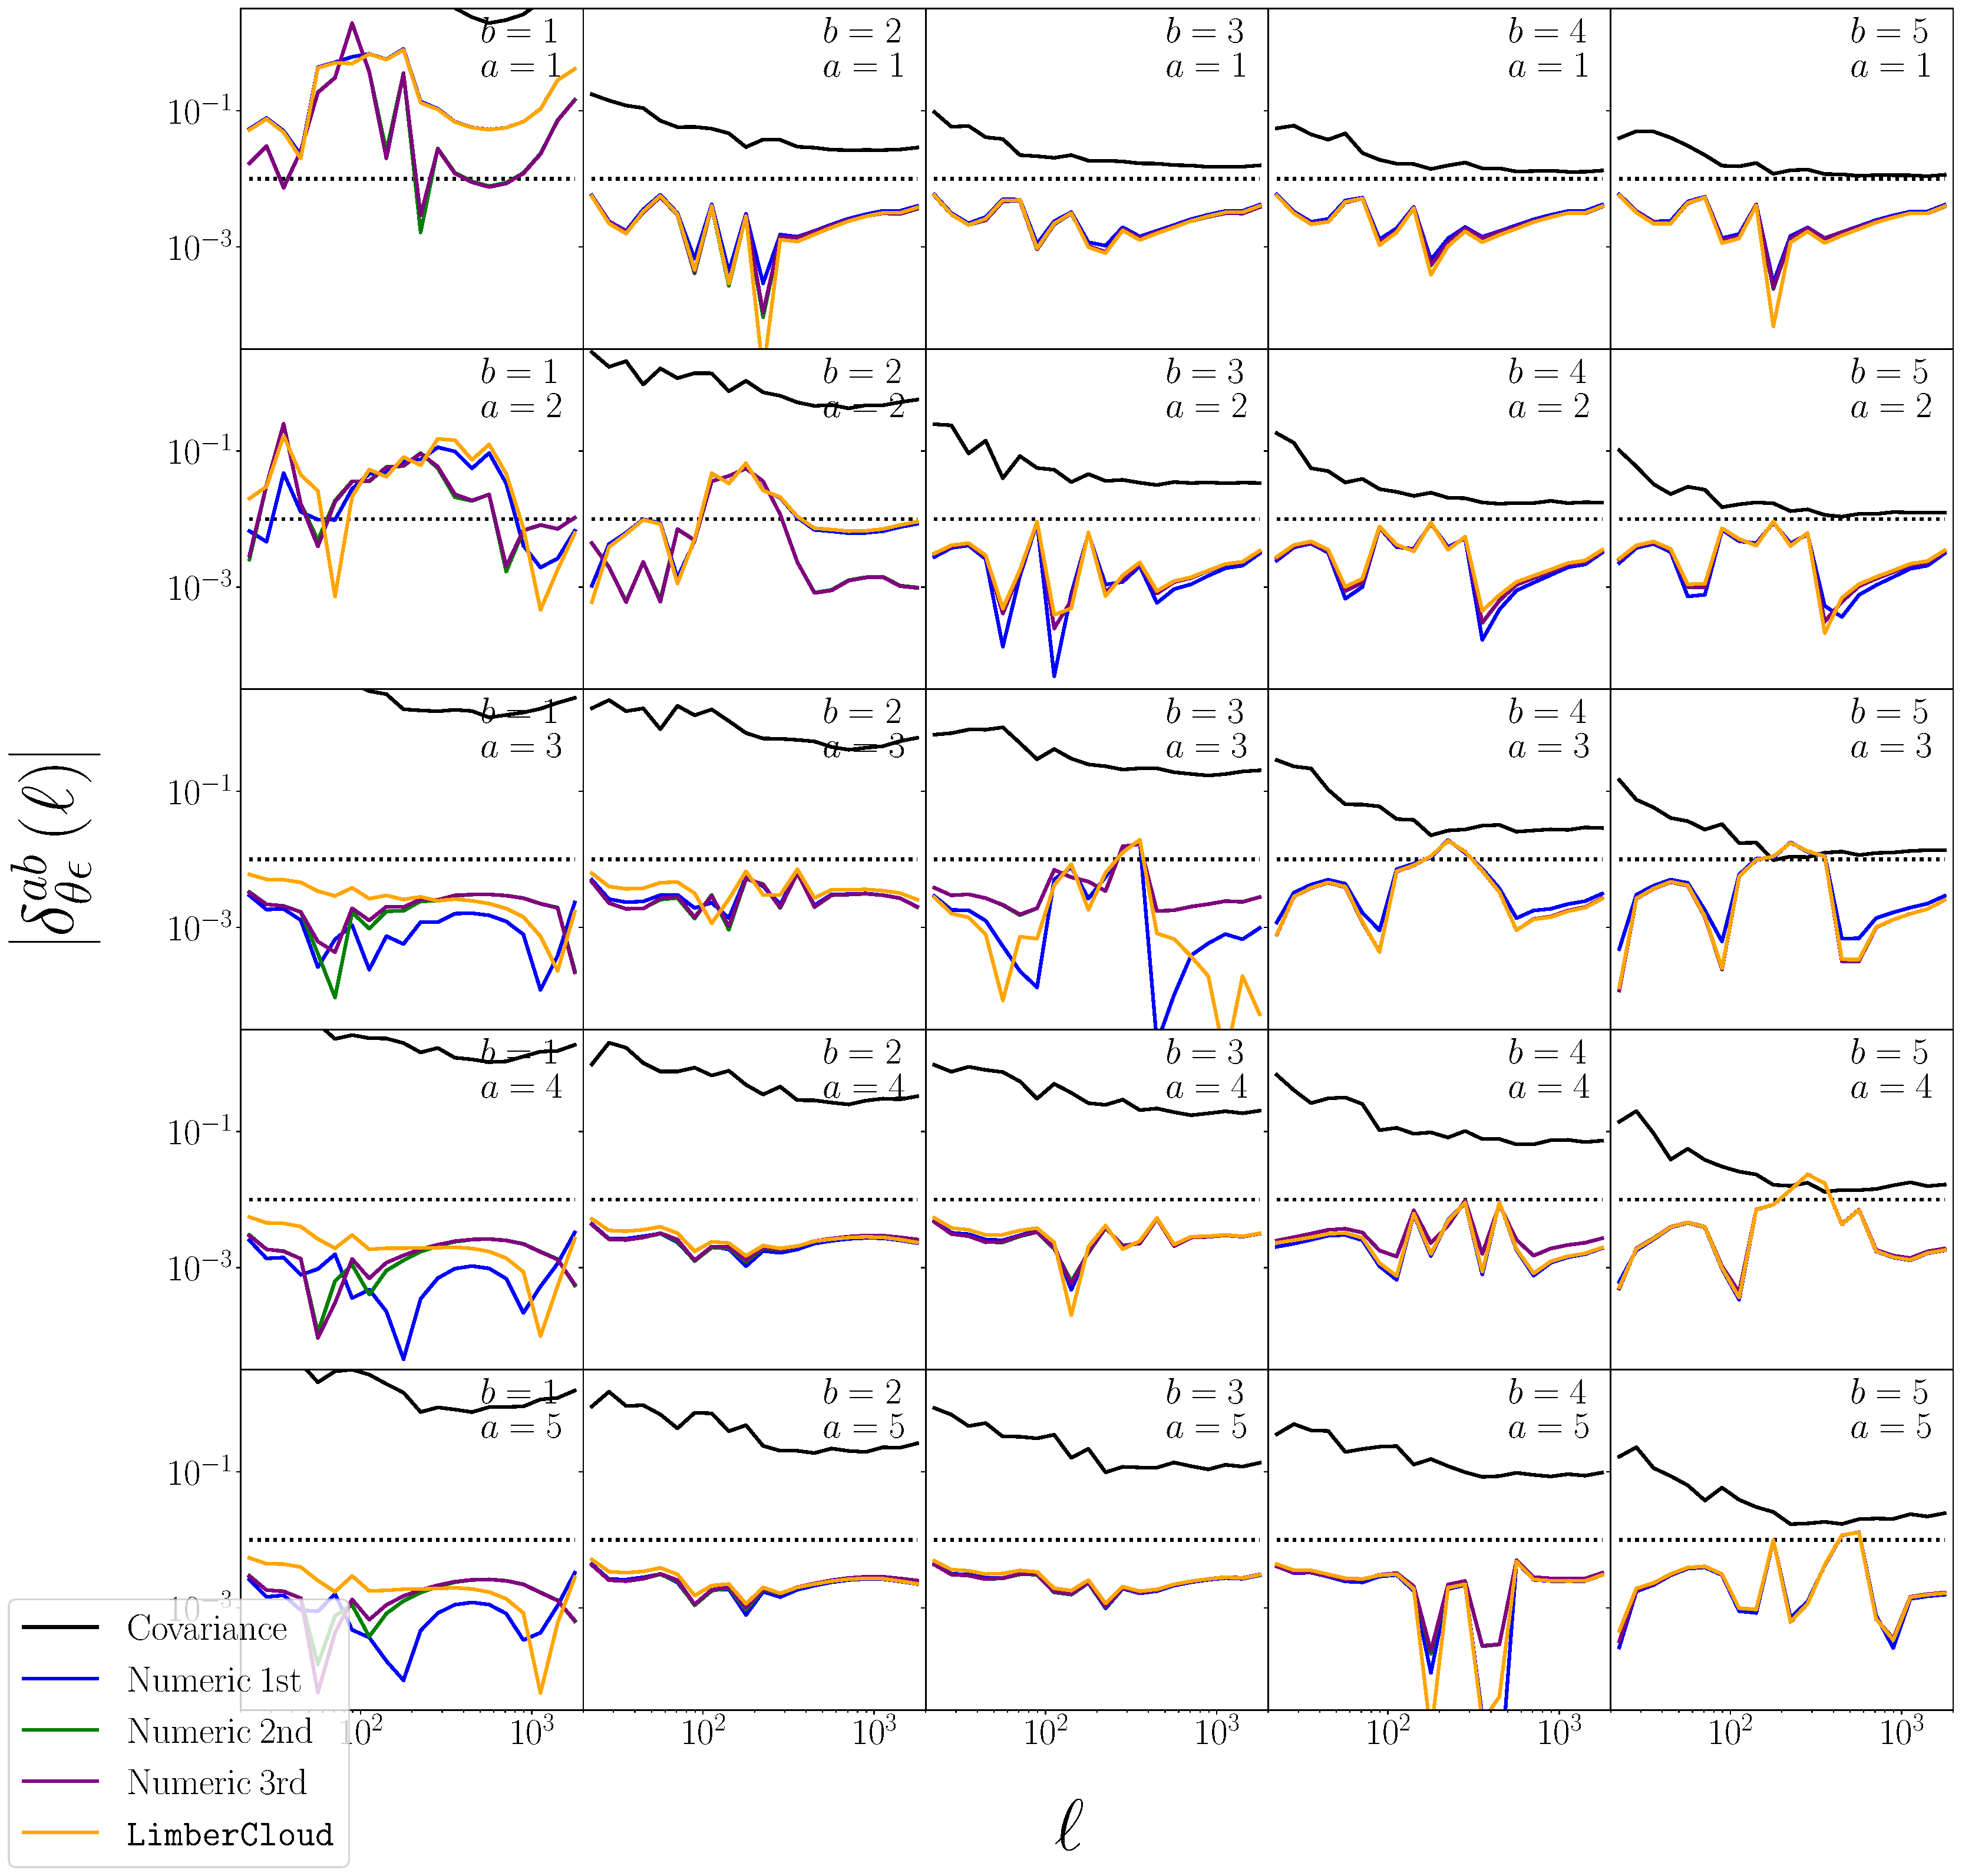
\includegraphics[width=0.95\textwidth]{figures/ERROR_TE_Y1.pdf}
    \caption{Absolute fractional error \(|\delta_{\theta\epsilon}^{ab}(\ell)|\) in the position--shape (galaxy--galaxy lensing) angular power spectra \(C_{\theta\epsilon}^{ab}(\ell)\) relative to \texttt{CCL}, shown for all 25 lens--source bin combinations of the LSST Y1 survey scenario. Conventions follow Figure~\ref{fig:5}. Elevated fractional errors visible in panels where the lens and source bins overlap in redshift (e.g.\ \(a = 1\), \(b = 1\) and \(a = 2\), \(b = 1\)) arise because the gravitational lensing signal \(C_\mathrm{g\gamma}\) is suppressed when the two populations share the same redshift range, leaving the observable dominated by intrinsic-alignment and magnification contributions; these bin pairs are not conventionally included in \(3\times2\,\mathrm{pt}\) analyses. For all standard bin combinations, the \texttt{LimberCloud} error is comfortably below both the one per cent line and the survey variance.}
    \label{fig:6}
\end{figure*}

\subsection{Position--position correlation} \label{sec:5.3}

The position--position angular power spectrum \(C_{\theta\theta}^{ab}(\ell)\) receives contributions from intrinsic galaxy--galaxy correlations and from magnification terms (Equation~\ref{eq:2.7}). For the dominant intrinsic clustering contribution \(C_\mathrm{gg}^{ab}(\ell)\), Table~\ref{tab:1} specifies \(A_\mathrm{gg}(\ell) = 1\) and both kernels of number-density type, so that \(r_u^{i,n} = r_v^{j,n} = r_\phi^{i,n}\). The interval tensor becomes
\begin{equation} \label{eq:5.9}
    B_\mathrm{gg}^{ij,n}(\ell) = \int_{\chi_n}^{\chi_{n+1}} \mathrm{d}\chi\; \frac{r_\phi^{i,n}(\chi)\,r_\phi^{j,n}(\chi)}{\chi^2}\, P_\mathrm{gg}\!\left[\frac{\ell+1/2}{\chi},\, z(\chi)\right],
\end{equation}
where \(P_\mathrm{gg}(k,z) = b_\mathrm{g}^2(k,z)\,P_{\delta\delta}(k,z)\) absorbs the galaxy bias. Since both kernel coefficients \(r_\phi^{i,n}\) are non-zero only for \(i \in \{n, n{+}1\}\) (Equation~\ref{eq:4.5}), \(B_\mathrm{gg}^{ij,n}\) has at most four non-zero entries per interval---three after symmetry---giving the maximally sparse tensor structure. The magnification cross-terms \(C_\mathrm{g\mu}^{ab}(\ell)\) and \(C_{\mu\mathrm{g}}^{ab}(\ell)\) each involve one number-density and one lensing convergence kernel, producing an eight-element mixed-sparsity structure, while the magnification auto-term \(C_{\mu\mu}^{ab}(\ell)\) uses \(r_\kappa^{i,n}\) on both legs and is dense in both indices.

Figure~\ref{fig:7} presents the validation for the position--position power spectra. In standard \(3\times2\,\mathrm{pt}\) analyses, only the auto-spectra (\(a = b\)) are conventionally included, so their accuracy is of primary importance. The auto-spectra are dominated by the intrinsic clustering contribution \(C_\mathrm{gg}\), which involves only \(r_\phi\) kernels and benefits from the simplest integral structure and maximal sparsity. For the majority of multipoles, the \texttt{LimberCloud} error in the auto-spectra lies at around the few times \(10^{-3}\) level. However, at certain multipole ranges the error can approach the diagonal of the survey covariance (solid curve), particularly for the highest-redshift bins where the statistical uncertainties are smallest relative to the signal. This behaviour reflects the sensitivity of galaxy clustering to the precise shape of the redshift distributions: because the number-density kernel \(W_\phi^a\) coincides directly with \(\phi^a(\chi)\), any interpolation-induced distortion of the distribution shape propagates without the smoothing provided by the lensing efficiency integral. Nevertheless, this numerical residual remains well below the level of current photometric redshift uncertainties, which dominate the systematic error budget for galaxy clustering and are themselves marginalised over in cosmological analyses. Furthermore, the multipoles at which the residual is most apparent fall close to or beyond the conventional linear-bias scale cut. The linear galaxy-bias model adopted throughout this work (Section~\ref{sec:3.2}) is theoretically reliable only for \(k \lesssim 0.1\,\mathrm{Mpc}^{-1}\) \citep{2022PhRvD.105l3518G}; at smaller scales, scale-dependent non-linear bias contributions dominate the modelling uncertainty over both the statistical and numerical residuals by a substantial margin. Current Stage-IV \(3\times2\,\mathrm{pt}\) analyses therefore impose a conservative scale cut, conventionally at \(k_{\mathrm{max}} \simeq 0.3\,h\,\mathrm{Mpc}^{-1}\) \citep{2009arXiv0912.0201L, 2022PhRvD.105b3520A}. Translated per tomographic bin via \(\ell_{\mathrm{max}}^a = k_{\mathrm{max}}\,\chi(z_{\mathrm{up}}^a) - 1/2\) at the upper redshift edge of each lens bin under the fiducial cosmology of Section~\ref{sec:3.1}, this yields \(\ell_{\mathrm{max}} \approx 320\) in the lowest lens bin (\(z_{\mathrm{up}} = 0.4\)) and \(\ell_{\mathrm{max}} \approx 780\) in the highest (\(z_{\mathrm{up}} = 1.2\)); the residual--covariance crossings visible in Figure~\ref{fig:7} lie close to or beyond this excluded regime. The argument is moreover insensitive to the precise cut: even an aggressive alternative such as \(k_{\mathrm{max}} \simeq 0.5\,\mathrm{Mpc}^{-1}\), accessible with hybrid effective field theory bias models \citep{2024JCAP...02..015N}, places the residuals well inside the bias-modelling-dominated regime. The piecewise-linear approximation error is therefore negligible in the context of realistic inference.

\begin{figure*}[!htbp]
    \centering
    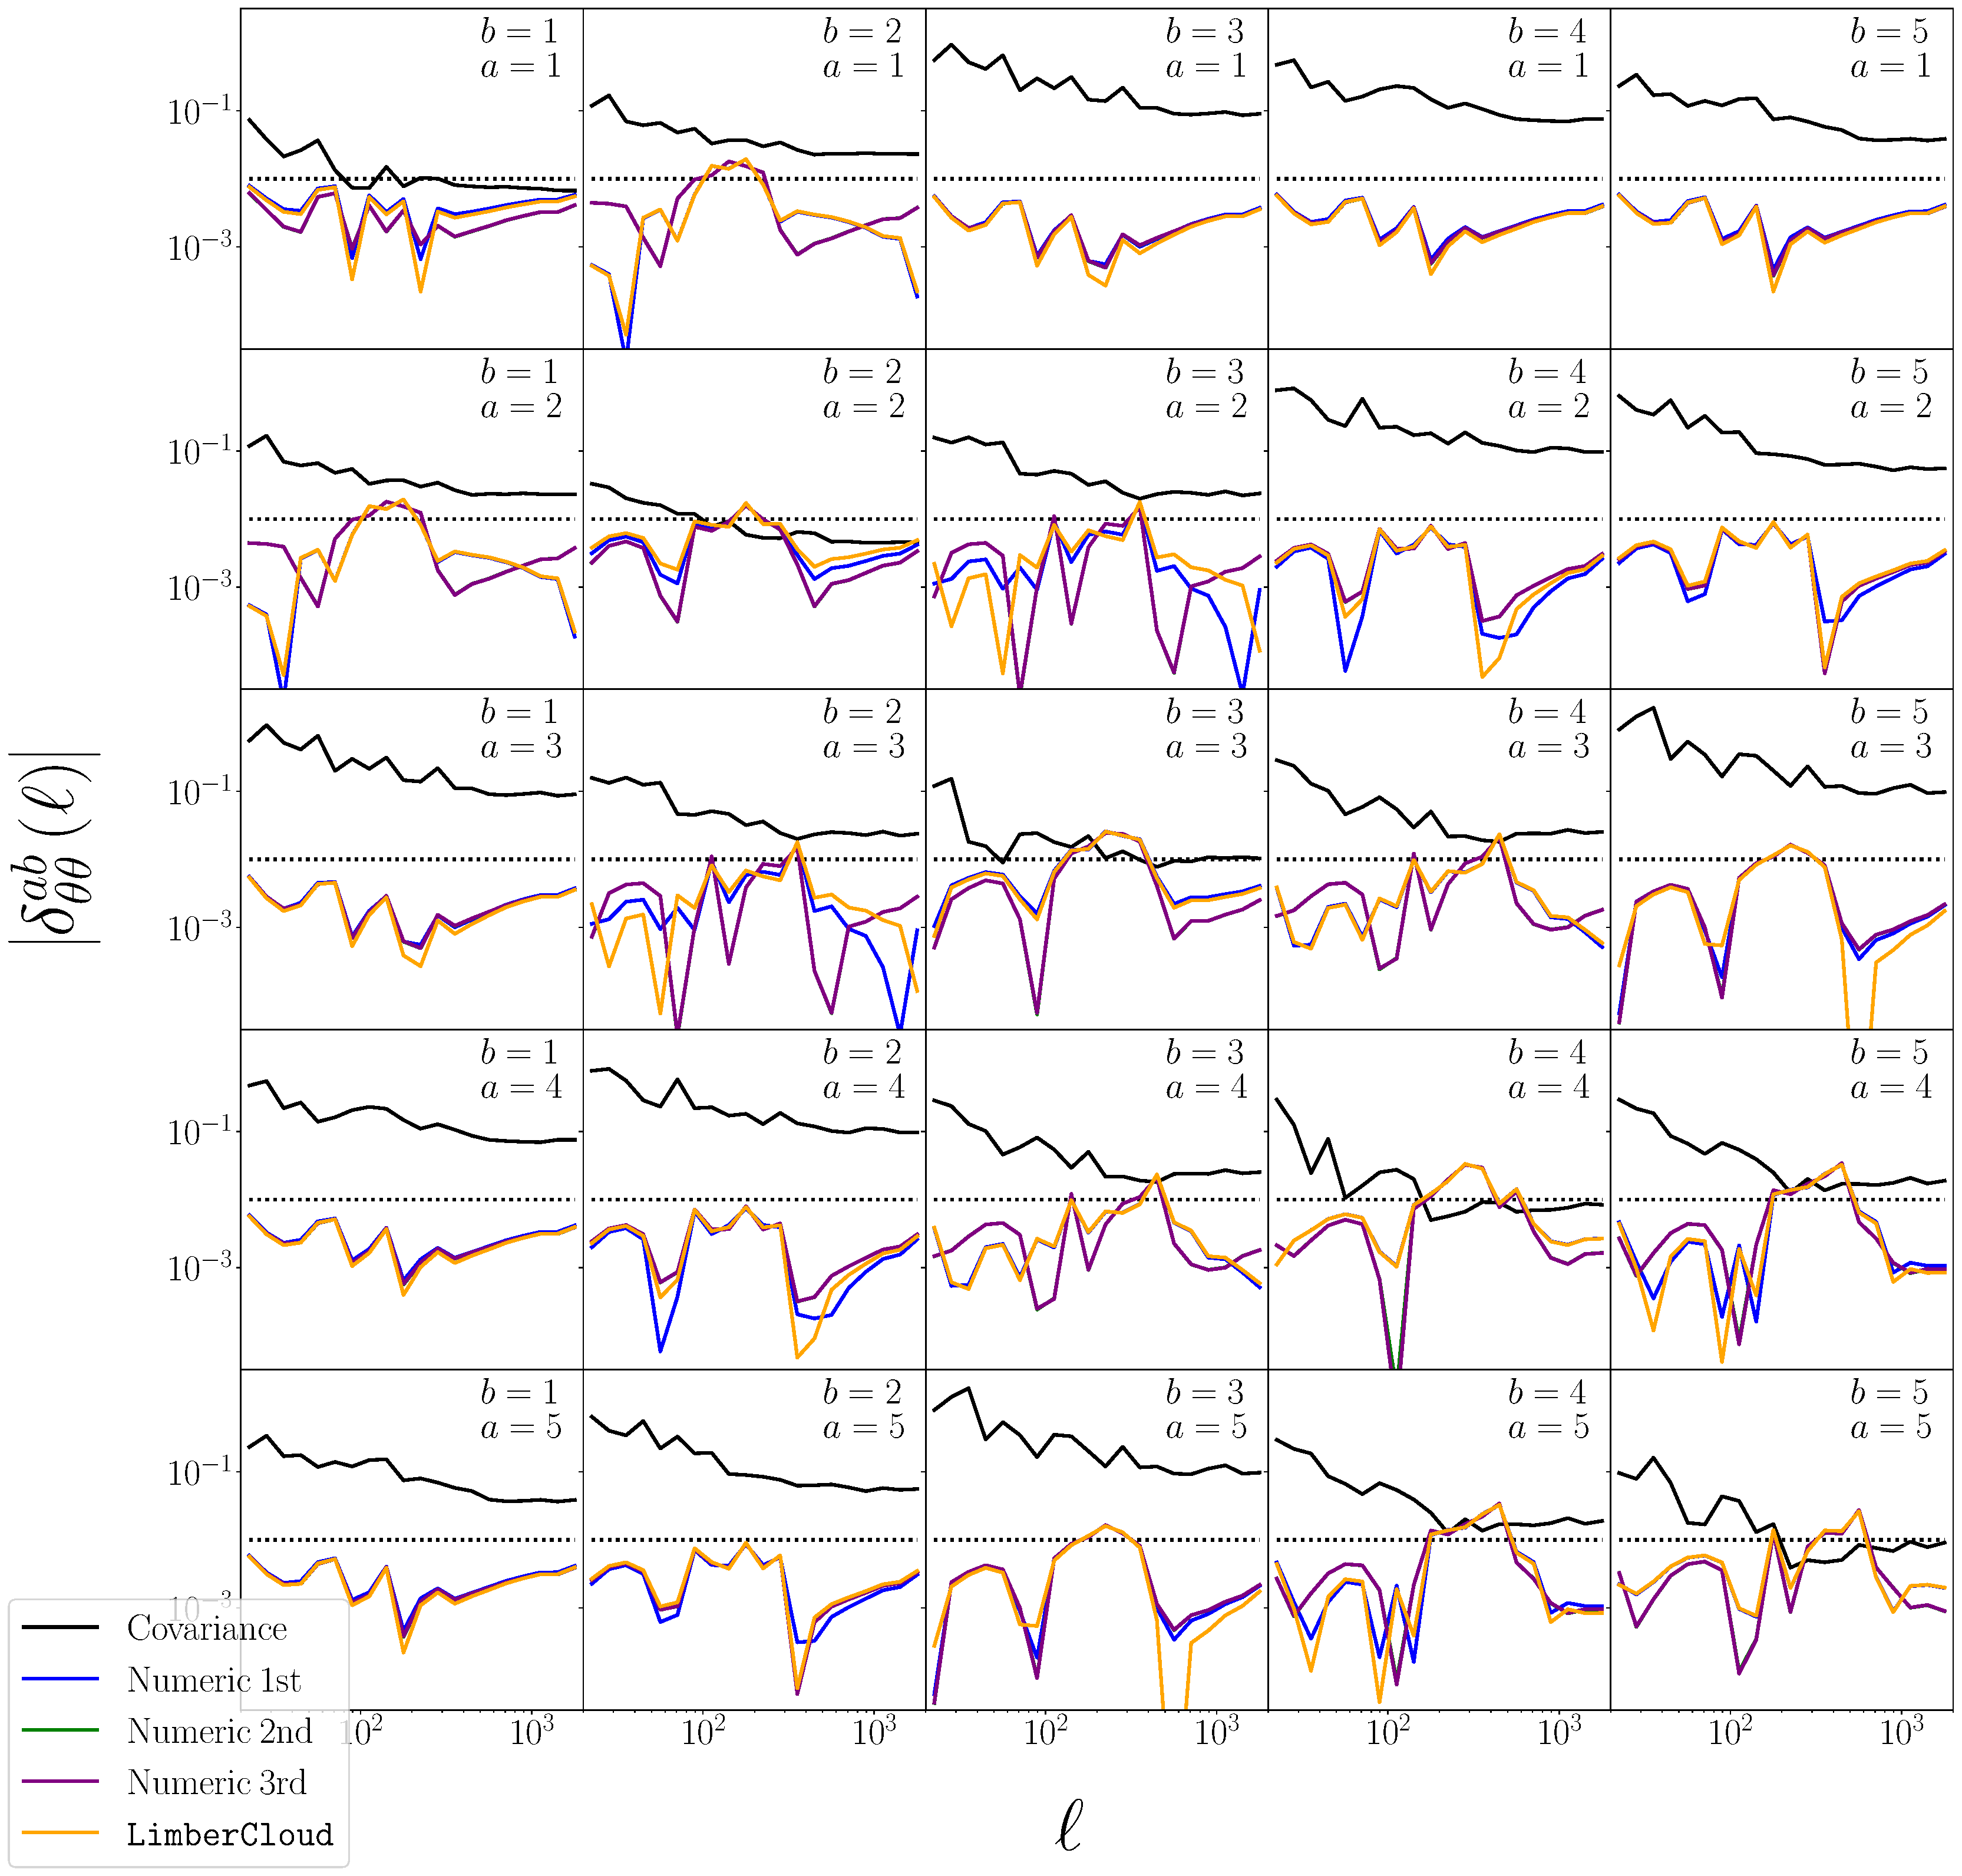
\includegraphics[width=0.95\textwidth]{figures/ERROR_TT_Y1.pdf}
    \caption{Absolute fractional error \(|\delta_{\theta\theta}^{ab}(\ell)|\) in the position--position (galaxy clustering) angular power spectra \(C_{\theta\theta}^{ab}(\ell)\) relative to \texttt{CCL}, shown for all 25 lens-bin combinations of the LSST Y1 survey scenario. Conventions follow Figure~\ref{fig:5}. The auto-spectra (diagonal panels), dominated by intrinsic galaxy clustering \(C_\mathrm{gg}\), typically achieve few times \(10^{-3}\) accuracy; at certain multipole ranges the error can approach the survey covariance level, reflecting the sensitivity of galaxy clustering to the precise shape of the redshift distributions. Cross-bin spectra for widely separated lens bins (e.g.\ \(a = 1\), \(b = 5\)) exhibit larger fractional errors because the observable is dominated by subdominant magnification contributions (\(C_\mathrm{g\mu}\), \(C_{\mu\mathrm{g}}\), \(C_{\mu\mu}\)); these spectra are not conventionally included in standard cosmological analyses and their statistical uncertainties (solid curve) are correspondingly large.}
    \label{fig:7}
    \end{figure*}

The off-diagonal panels (\(a \ne b\)) exhibit larger fractional errors for widely separated lens bins (e.g.\ \(a = 1\), \(b = 5\)), reaching \(\sim 10^{-2}\)--\(10^{-1}\) at certain multipoles. This occurs because the intrinsic clustering signal \(C_\mathrm{gg}\) is negligible for non-overlapping bins, leaving the observable dominated by the much fainter magnification contributions (\(C_\mathrm{g\mu}\), \(C_{\mu\mathrm{g}}\), \(C_{\mu\mu}\)). These cross-bin spectra are not conventionally included in cosmological analyses and their statistical uncertainties are correspondingly large.

